\chapter{Proyecto}

\section{Introducción}

\begin{figure}[th!]
	\centering
	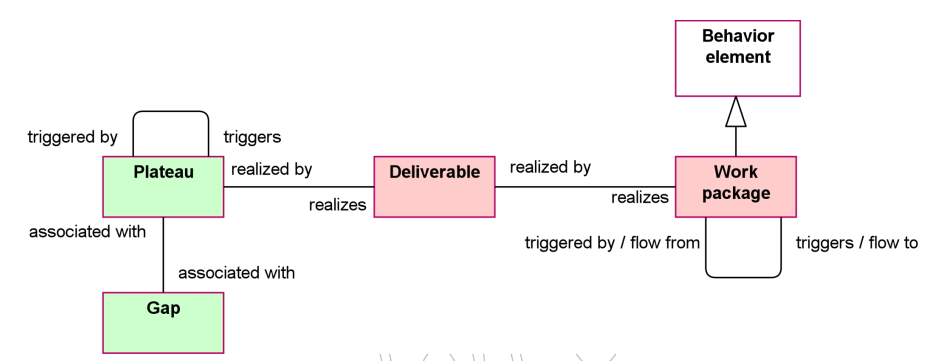
\includegraphics[width=1\linewidth]{arquitectura/imagenes/capaProyecto}
	\caption{Capa Proyecto}
	\label{modelo capa proyecto}
\end{figure}
Conceptualmente, la capa de proyecto es similar a un proceso de negocio, en el sentido de que consiste en un conjunto de tareas relacionadas causalmente, dirigidas a producir un resultado bien definido. Sin embargo, la capa de proyecto es un proceso único. Sin embargo la capa de proyecto se puede describir de una manera muy similar a la descripción de un proceso.

\newpage

\section{Punto de Vista de Proyecto}

\subsection{Modelo}
\begin{figure}[th!]
	\centering
	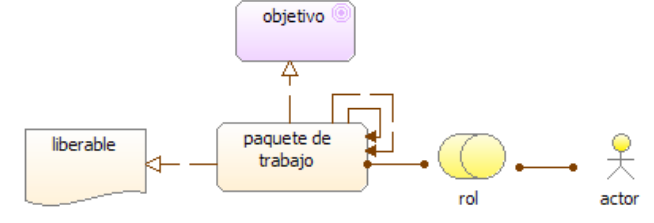
\includegraphics[width=0.7\linewidth]{arquitectura/imagenes/modeloProyecto}
	\caption{Metamodelo Punto de Vista Proyecto}
	\label{metamodelo proyecto}
\end{figure}
Un punto de vista del proyecto se utiliza principalmente para modelar la gestión del cambio de arquitectura. La "   arquitectura" del proceso de migración, desde una situación antigua (arquitectura de la empresa estatal actual) hasta una nueva situación deseada (arquitectura empresarial estatal objetivo) tiene consecuencias significativas en la estrategia de crecimiento a medio y largo plazo y en el proceso de toma de decisiones.

\subsection{Caso de estudio}

\begin{figure}[th!]
	\centering
	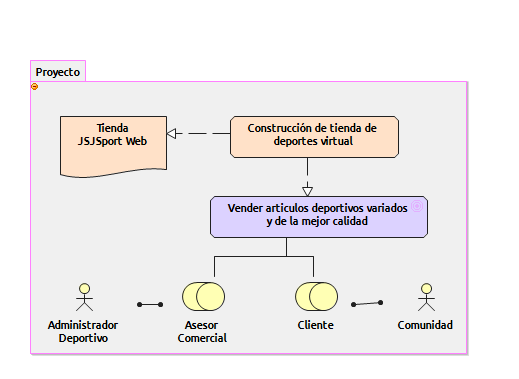
\includegraphics[width=0.8\linewidth]{arquitectura/imagenes/PuntoVistaProyecto}
	\caption{Modelo Punto de Vista Proyecto}
	\label{modelo proyecto}
\end{figure}

En la figura \ref{modelo proyecto} se puede observar que el paquete de trabajo es la construcción de la tienda de deportes virtual para JSJSports Web lo cual es el entregable de todo el proyecto, es decir este es el producto o resultado final al que se espera llegar, con el paquete de trabajo se busca cumplir el objetivo e vender artículos deportivos de la mejor calidad, este proceso a su vez involucra dos roles, el primero es el de asesor comercial que es interpretado por un administrador deportivo que tenga los conocimientos necesarios, el último rol es el de cliente, este rol es muy importante puesto que representa a toda la comunidad que accede a la tienda virtual.

\newpage

\section{Punto de Vista de Migración}

\subsection{Modelo}

\begin{figure}[th!]
	\centering
	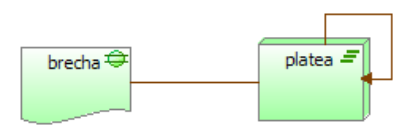
\includegraphics[width=0.8\linewidth]{arquitectura/imagenes/modeloMigracion}
	\caption{Metamodelo Punto de Vista Migración}
	\label{metamodelo migracion}
\end{figure}
El punto de vista de la migración implica modelos y conceptos que pueden usarse para especificar la transición de una arquitectura existente a una arquitectura deseada.

\subsection{Caso de estudio}

\begin{figure}[th!]
	\centering
	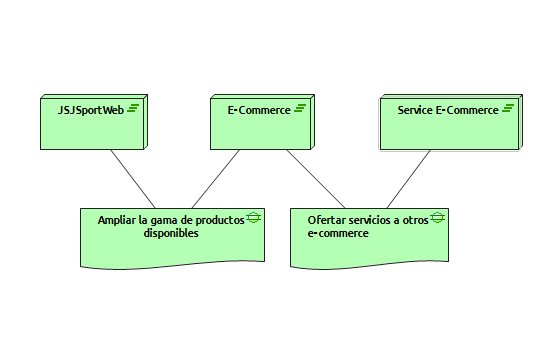
\includegraphics[width=0.8\linewidth]{arquitectura/imagenes/PuntoVistaMigracion}
	\caption{Modelo Punto de Vista Migración}
	\label{modelo migracion}
\end{figure}

En este punto de vista podemos ver la arquitectura que se ha venido modelando hasta el momento que se ve representada en el hito de JSJSports web, como equipo de trabajo hemos visto y planteado como trabajo futuro 2 arquitecturas diferentes una consecuencia de la otra, la primera de estas es convertir a JSJSports web en una plataforma e-commerce general que no solo se aplique a artículos deportivos sino que en esta se pueda ofertar cualquier tipo de artículo y se cuente con un vendedor que brinde soporte al cliente durante el proceso de compra, para esto es necesario aumentar el número de módulos y de productos disponibles, es decir diversificar la página.\newline
Para el caso de el último de los hitos, la arquitectura deseada busca hacer que JSJSports Web proporcione un servicio para diferentes páginas, es decir que no sea necesario que el cliente se encuentre en el dominio de la página sino que este pueda consultar productos por medio de otras o de terceros.

\newpage

\section{Punto de Vista de Implementación y Migración}

\subsection{Modelo}

\begin{figure}[th!]
	\centering
	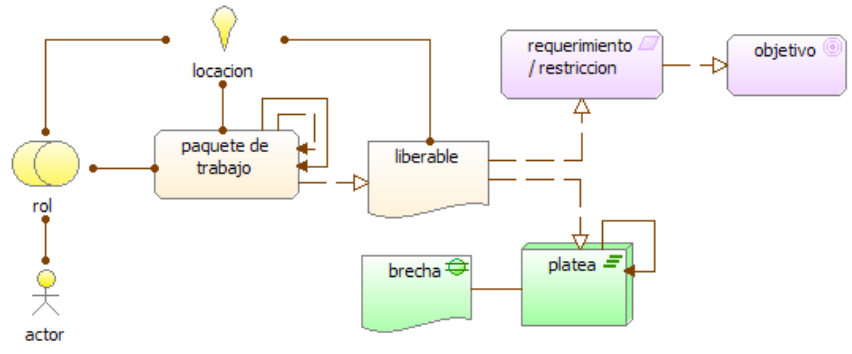
\includegraphics[width=0.7\linewidth]{arquitectura/imagenes/modeloMigracionImplementacion}
	\caption{Metamodelo Punto de Vista Migración e Implementación}
	\label{metamodelo migracion e implementacion}
\end{figure}
El punto de vista de migración e implementación se utiliza para relacionar programas y proyectos con las partes de la arquitectura que implementan. Esta visión permite modelar el alcance de los programas, proyectos, actividades del proyecto en términos de las mesetas que se realizan o los elementos de arquitectura individuales que se ven afectados. Además, la forma en que se afectan los elementos puede indicarse anotando las relaciones.
\subsection{Caso de estudio}

\begin{figure}[th!]
	\centering
	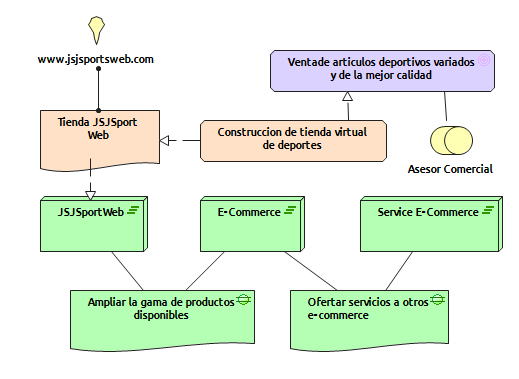
\includegraphics[width=0.8\linewidth]{arquitectura/imagenes/PuntoVistaMigracionImplementacion}
	\caption{Modelo Punto de Vista Migración e Implementación}
	\label{Modelo migracion e implementacion}
\end{figure}

En la figura \ref{Modelo migracion e implementacion} se puede observar el punto de vista de Migración e implementación que une los puntos de vista de las figuras  \ref{modelo proyecto} y \ref{modelo migracion}, aquí se unen estos puntos de vista por medio del entregable del proyecto y el la primer arquitectura hito puesto que ambos referencian a la tienda de JSJSports que se modela, además se especifica que todo esto se hará bajo el dominio de www.JSJSportsWeb.com.
\newpage

